\chapter{Apéndice B. Herramientas AHP utilizadas en el Diseño del Sistema.} 

\newpage
\begin{figure}[H]
	\centering
	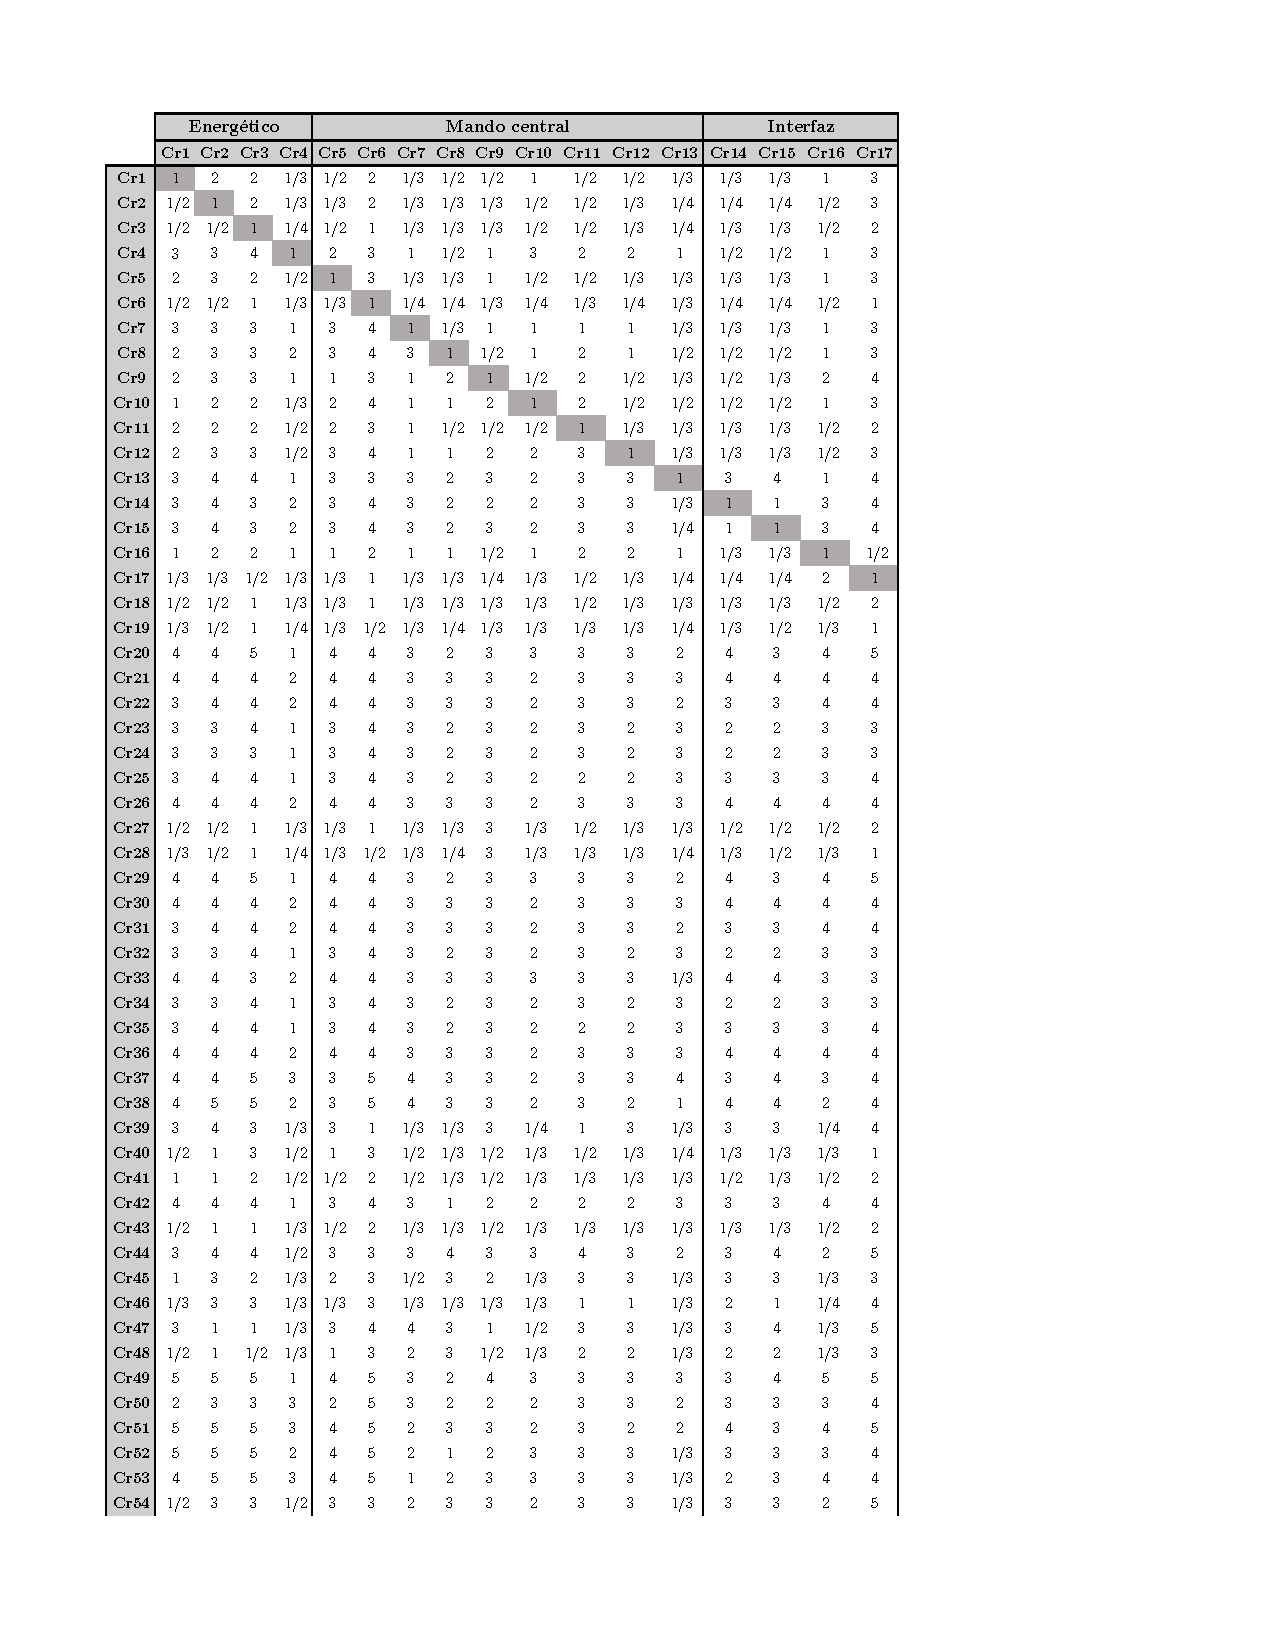
\includegraphics[width=16cm]{imagenes/MNormal1Ex}
	\caption{Matriz de criterios de los módulos energético, mando central e intefaz.}
	\label{fig:MNormal1Ex}
\end{figure}

\newpage
\begin{figure}[H]
\centering
	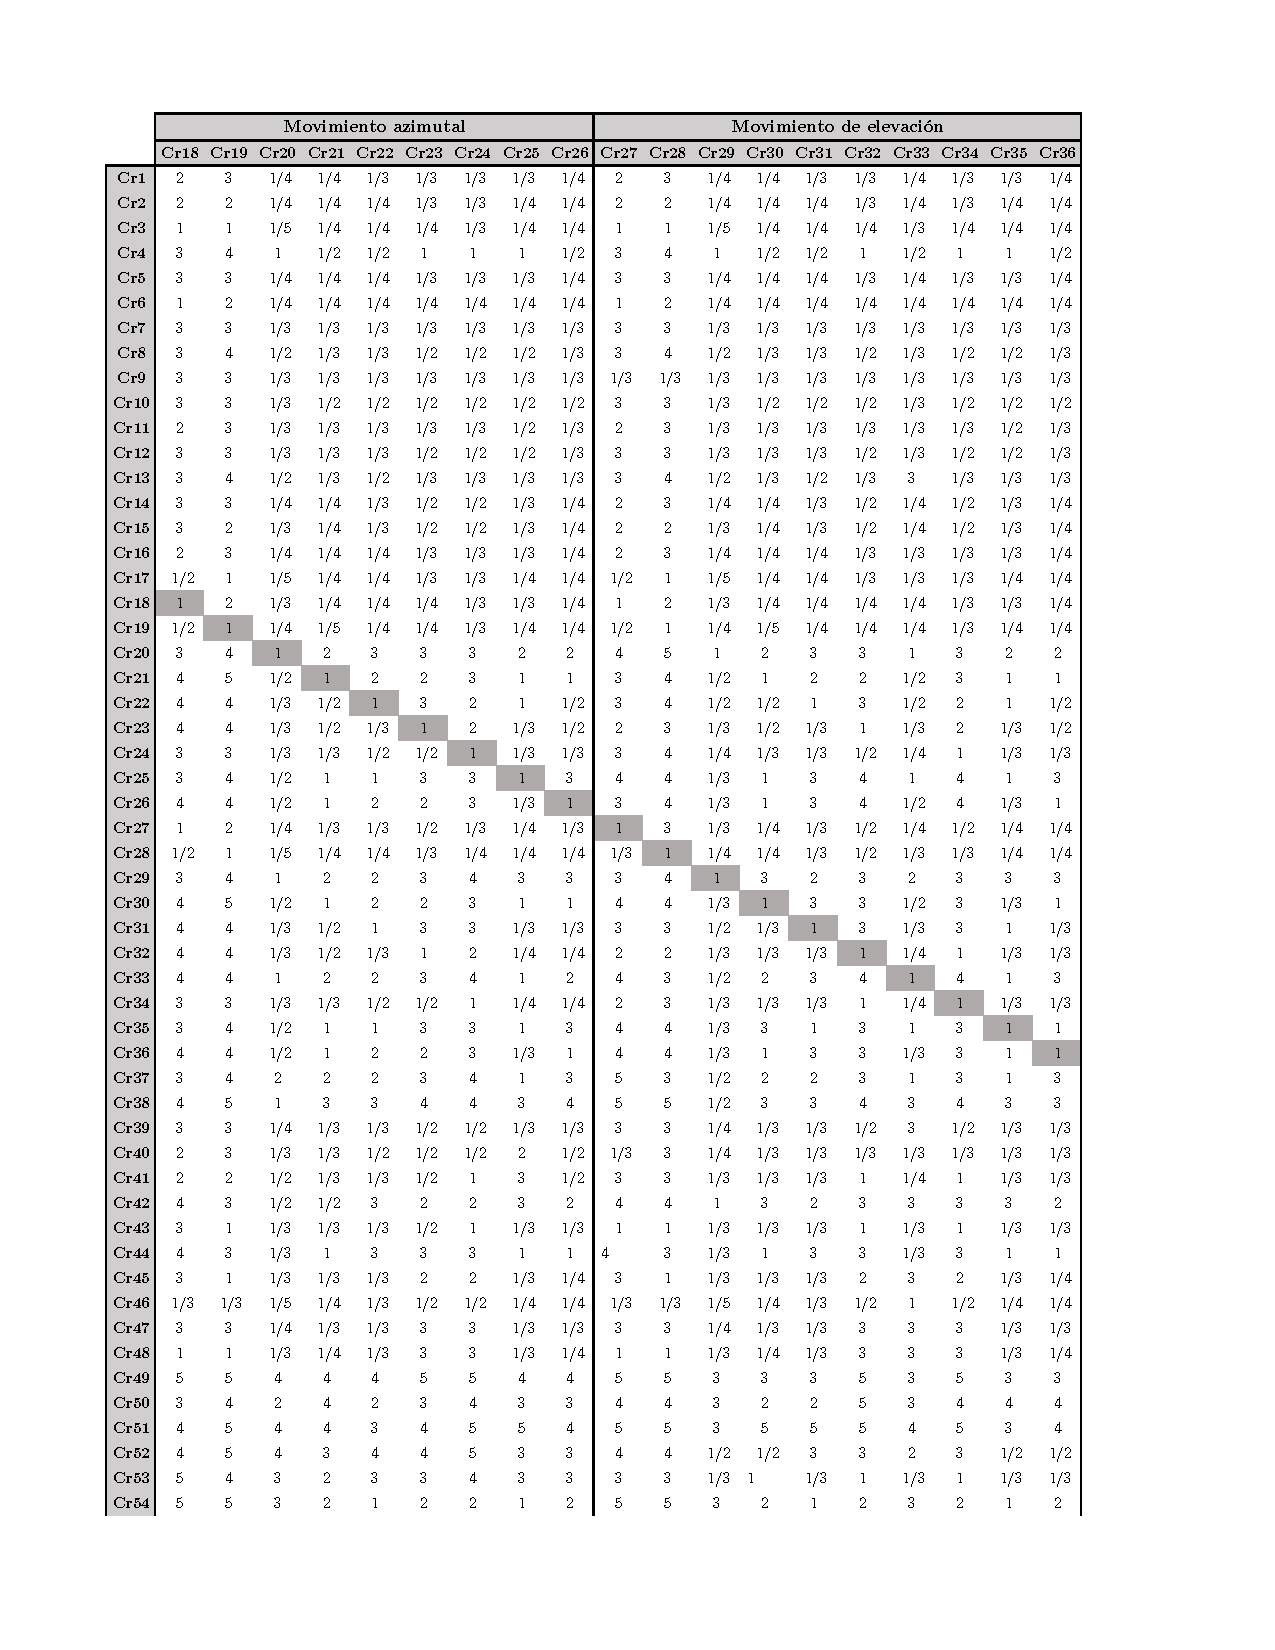
\includegraphics[width=16cm]{imagenes/MNormal2Ex}
	\caption{Matriz de criterios de los módulos movimiento azimutal y de elevación.}
	\label{fig:MNormal2Ex}
\end{figure}

\newpage
\begin{figure}[H]
	\centering
	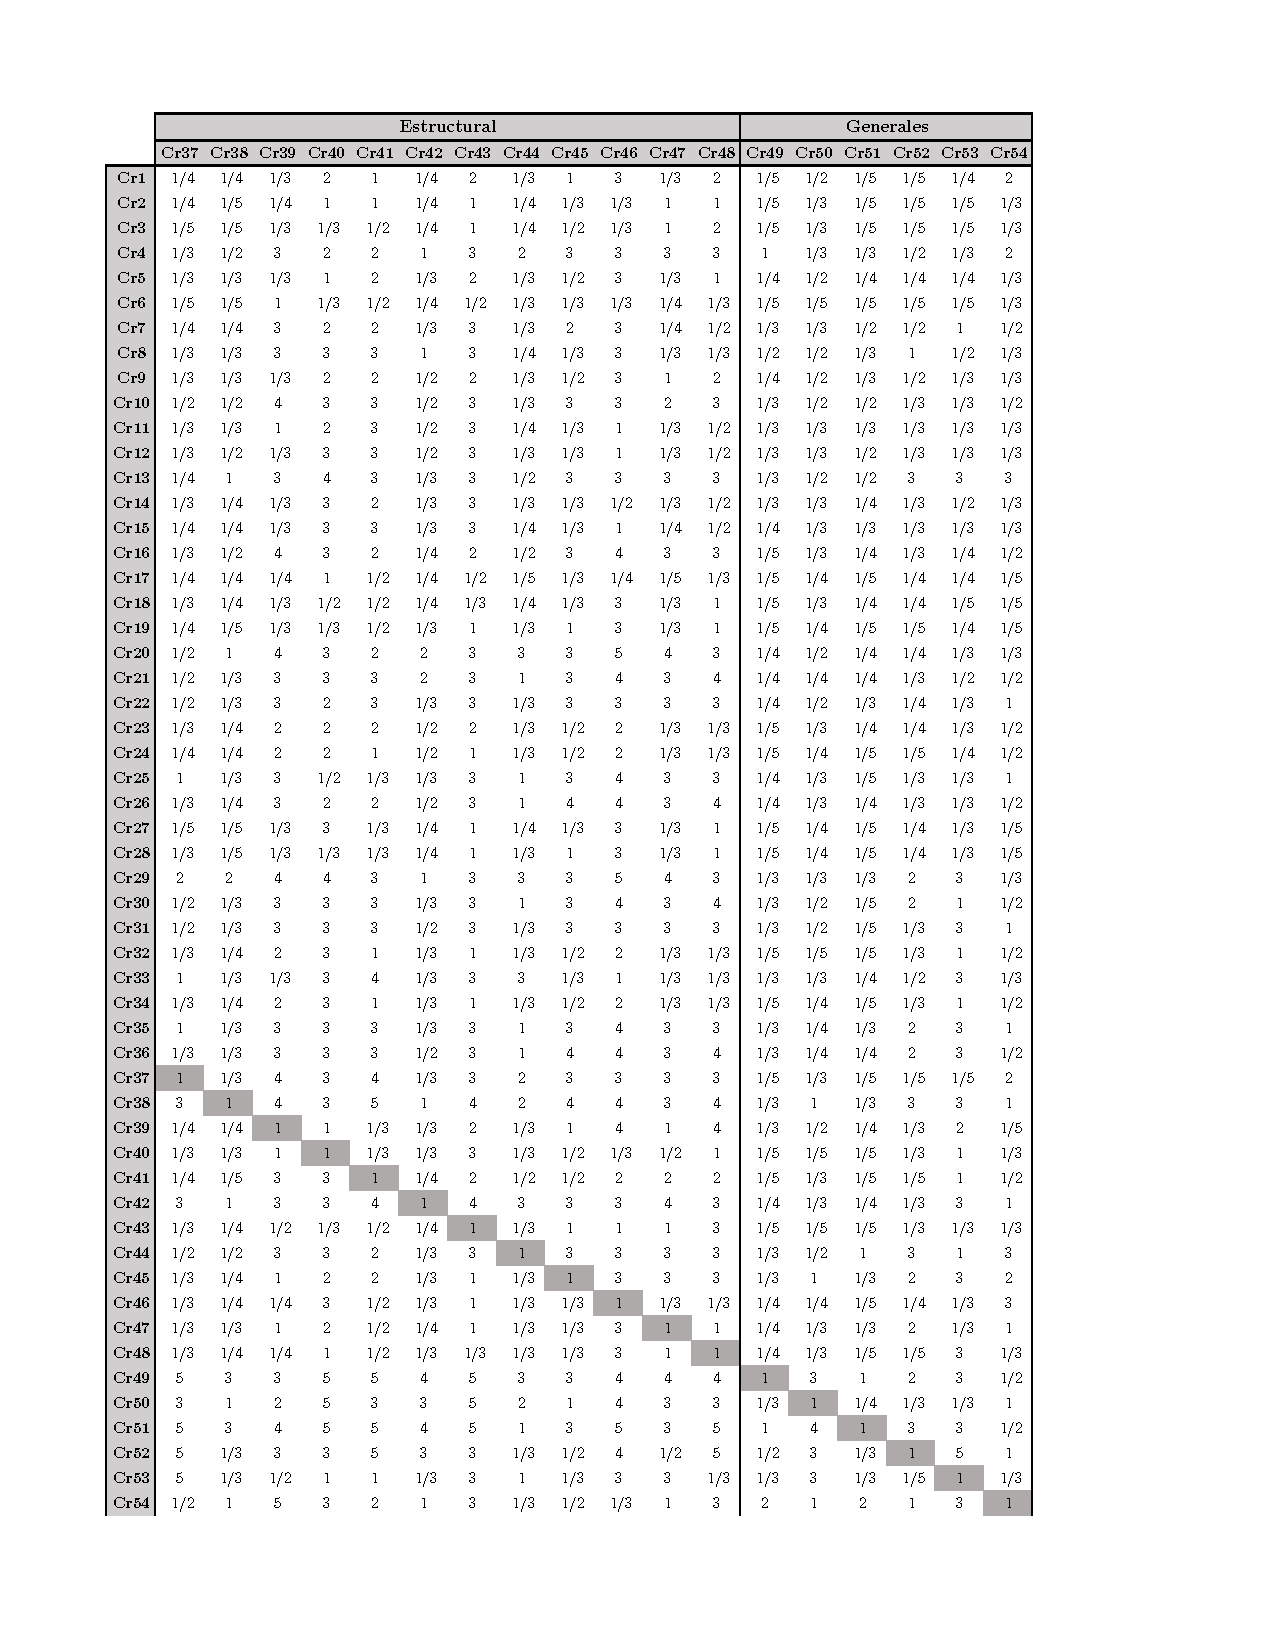
\includegraphics[width=16cm]{imagenes/MNormal3Ex}
	\caption{Matriz de criterios del módulo estructural y generales.}
	\label{fig:MNormal3Ex}
\end{figure}

\newpage
\begin{figure}[H]
	\centering
	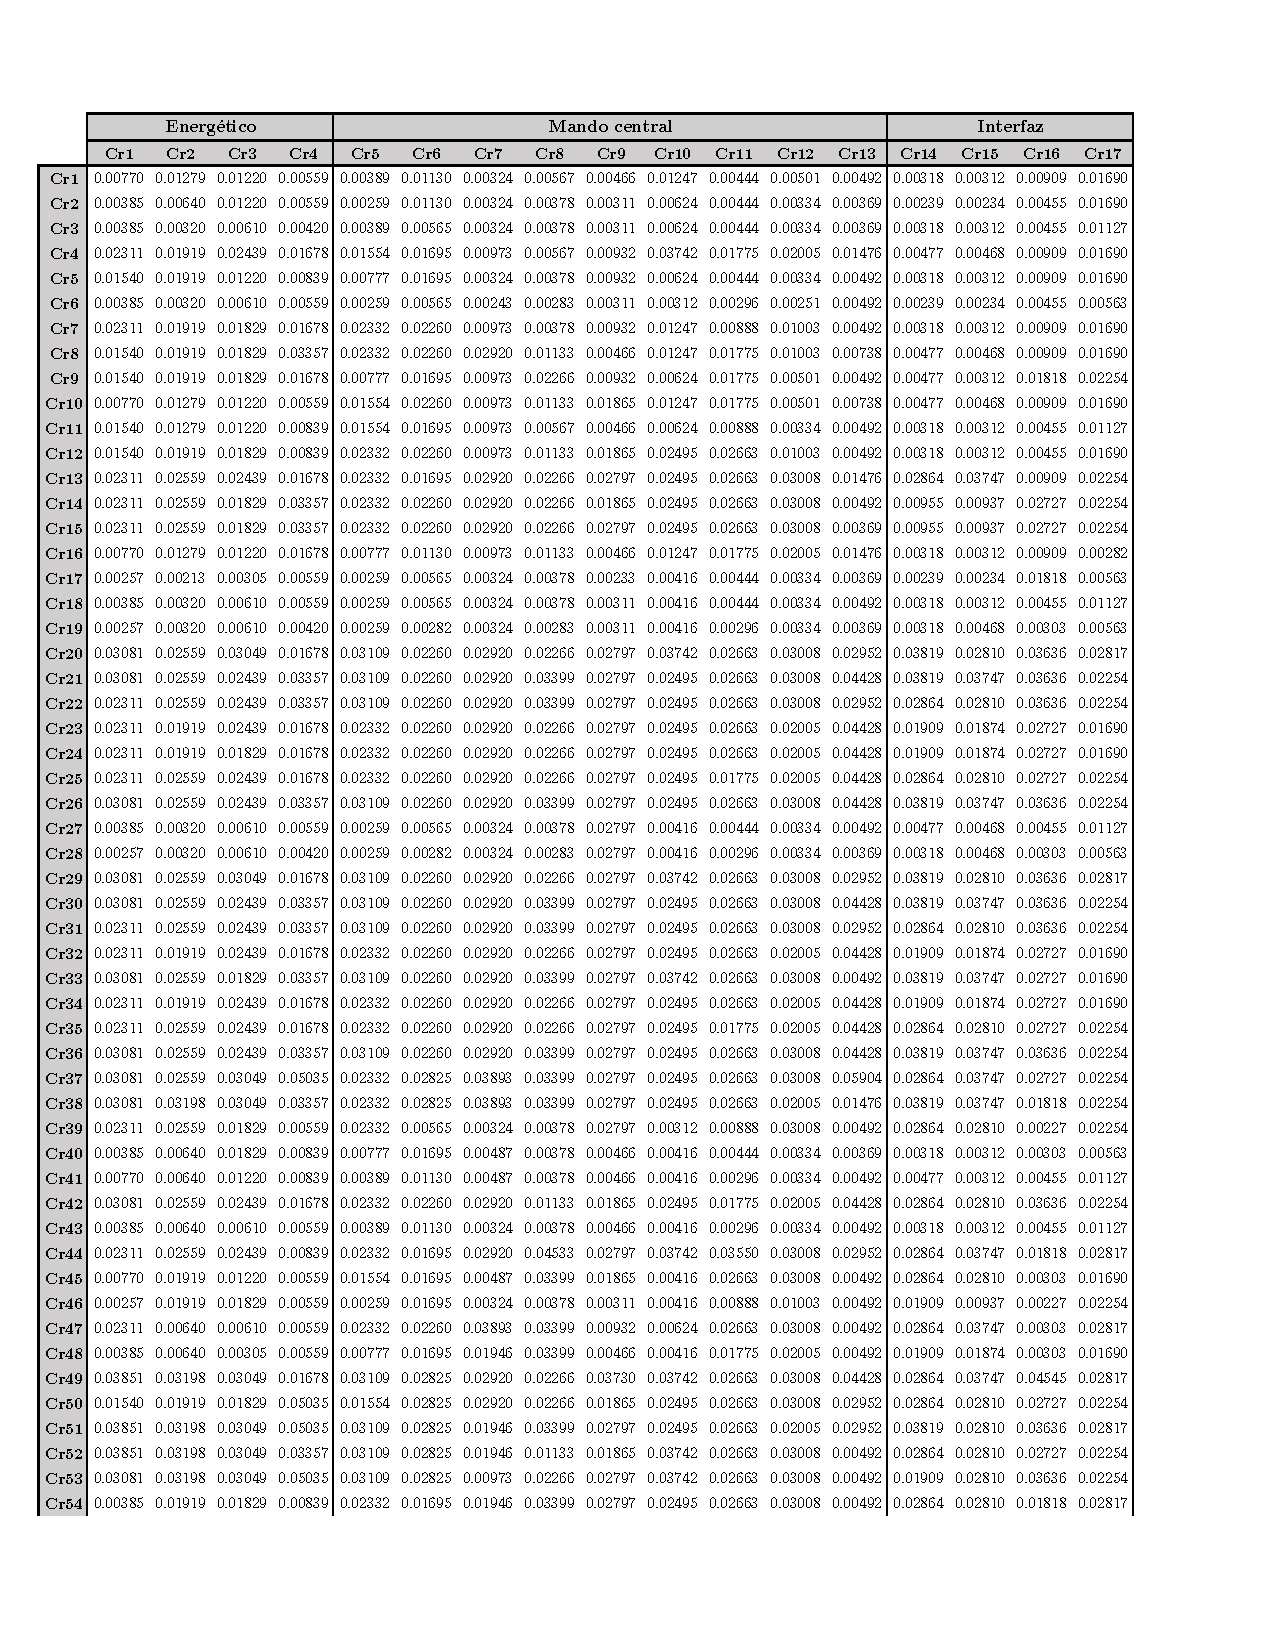
\includegraphics[width=16cm]{imagenes/MNormalizada1Ex}
	\caption{Matriz de criterios normalizada de los módulos energético, mando central e intefaz.}
	\label{fig:MNormalizada1Ex}
\end{figure}

\newpage
\begin{figure}[H]
	\centering
	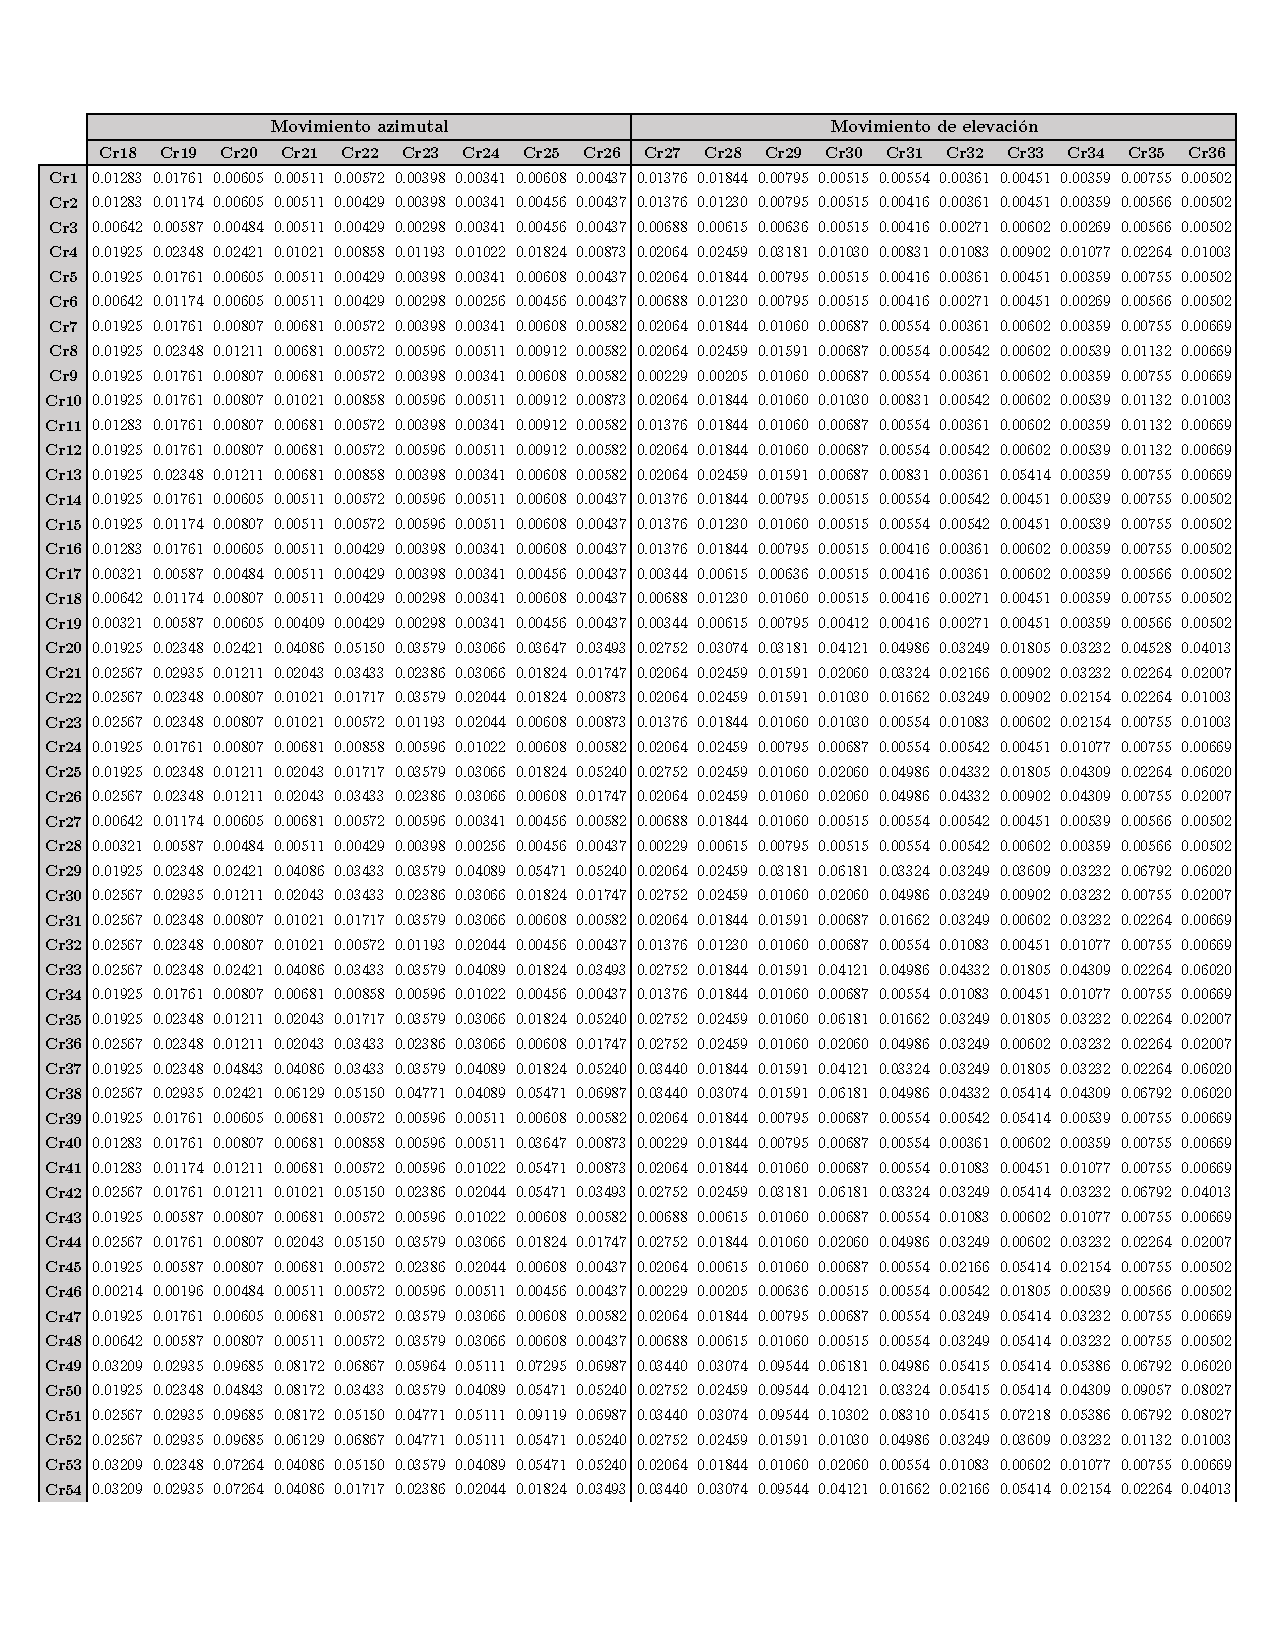
\includegraphics[width=15.5cm]{imagenes/MNormalizada2Ex}
	\caption{Matriz de criterios normalizada de los módulos movimiento azimutal y de elevación.}
	\label{fig:MNormalizada2Ex}
\end{figure}

\newpage
\begin{figure}[H]
	\centering
	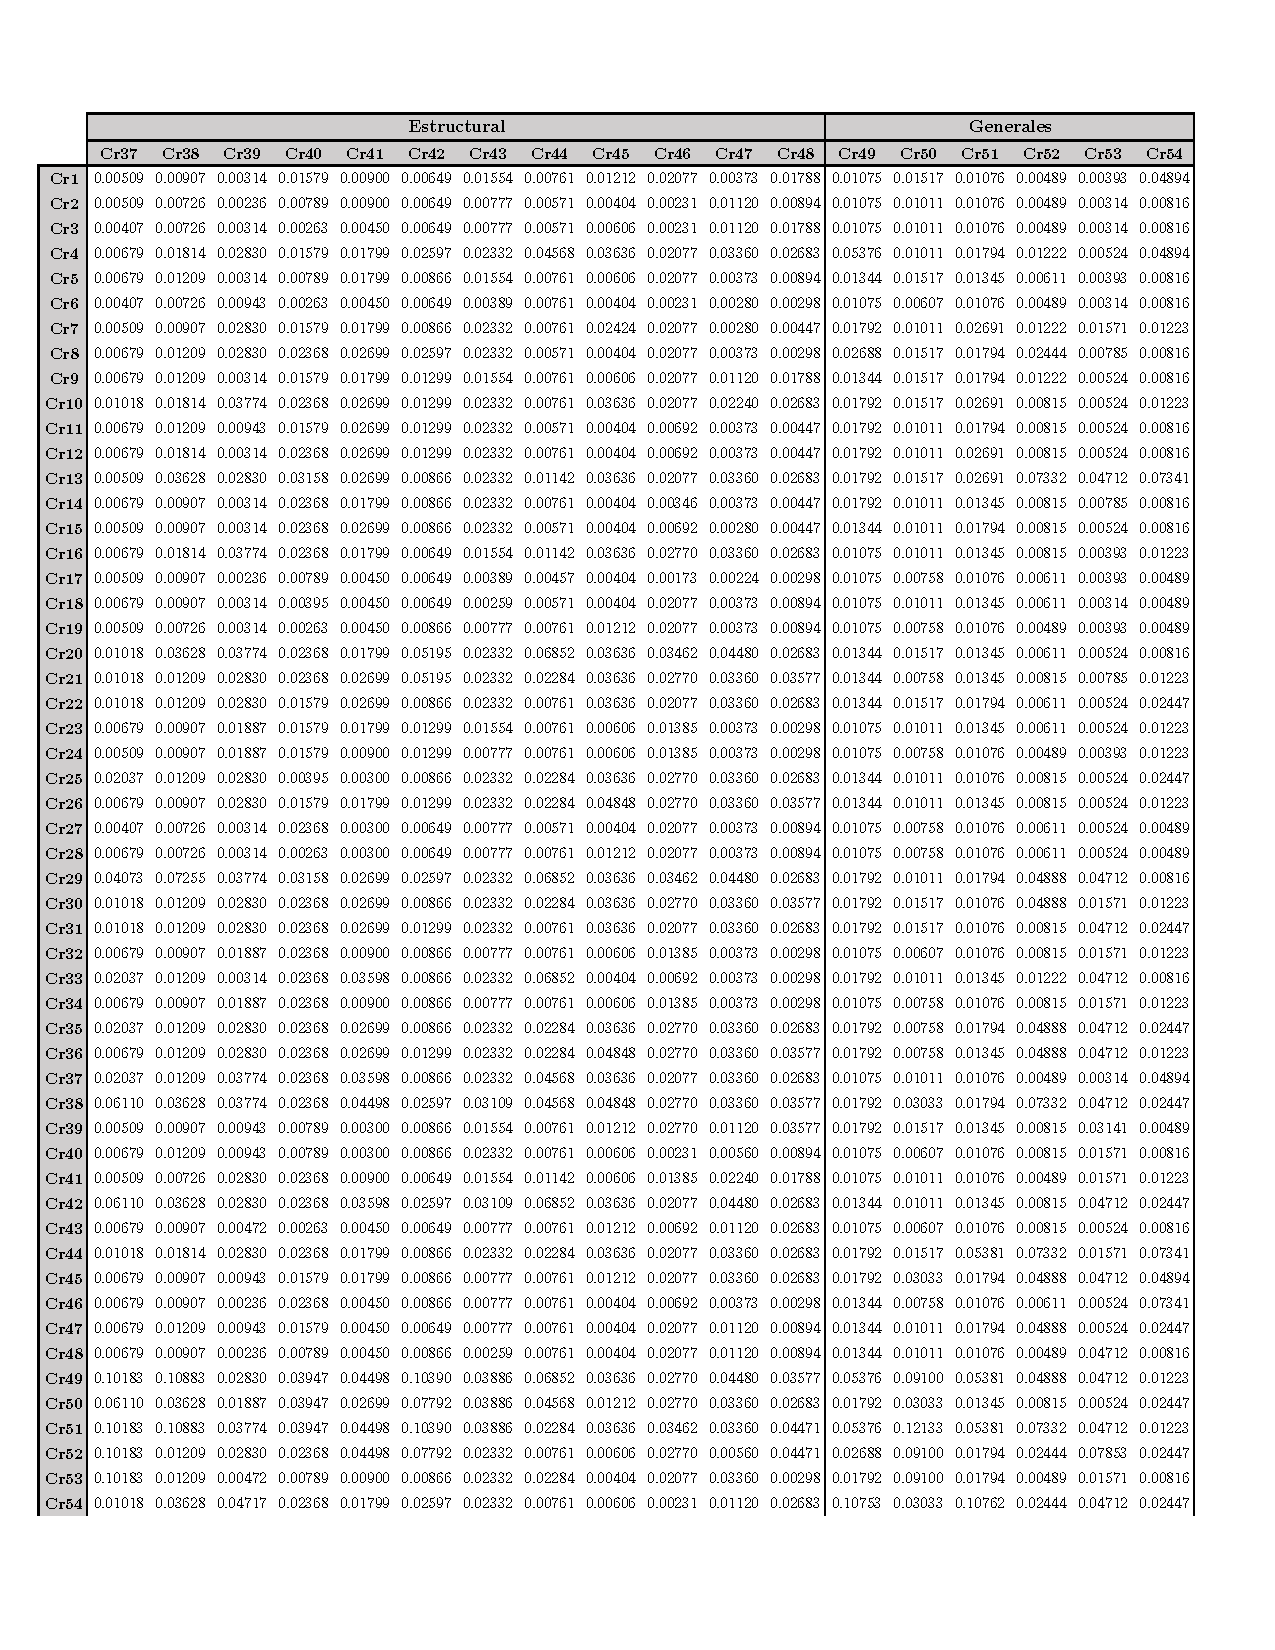
\includegraphics[width=15cm]{imagenes/MNormalizada3Ex}
	\caption{Matriz de criterios normalizada del módulo estructural y generales.}
	\label{fig:MNormalizada3Ex}
\end{figure}

\newpage
\begin{figure}[H]
	\centering
	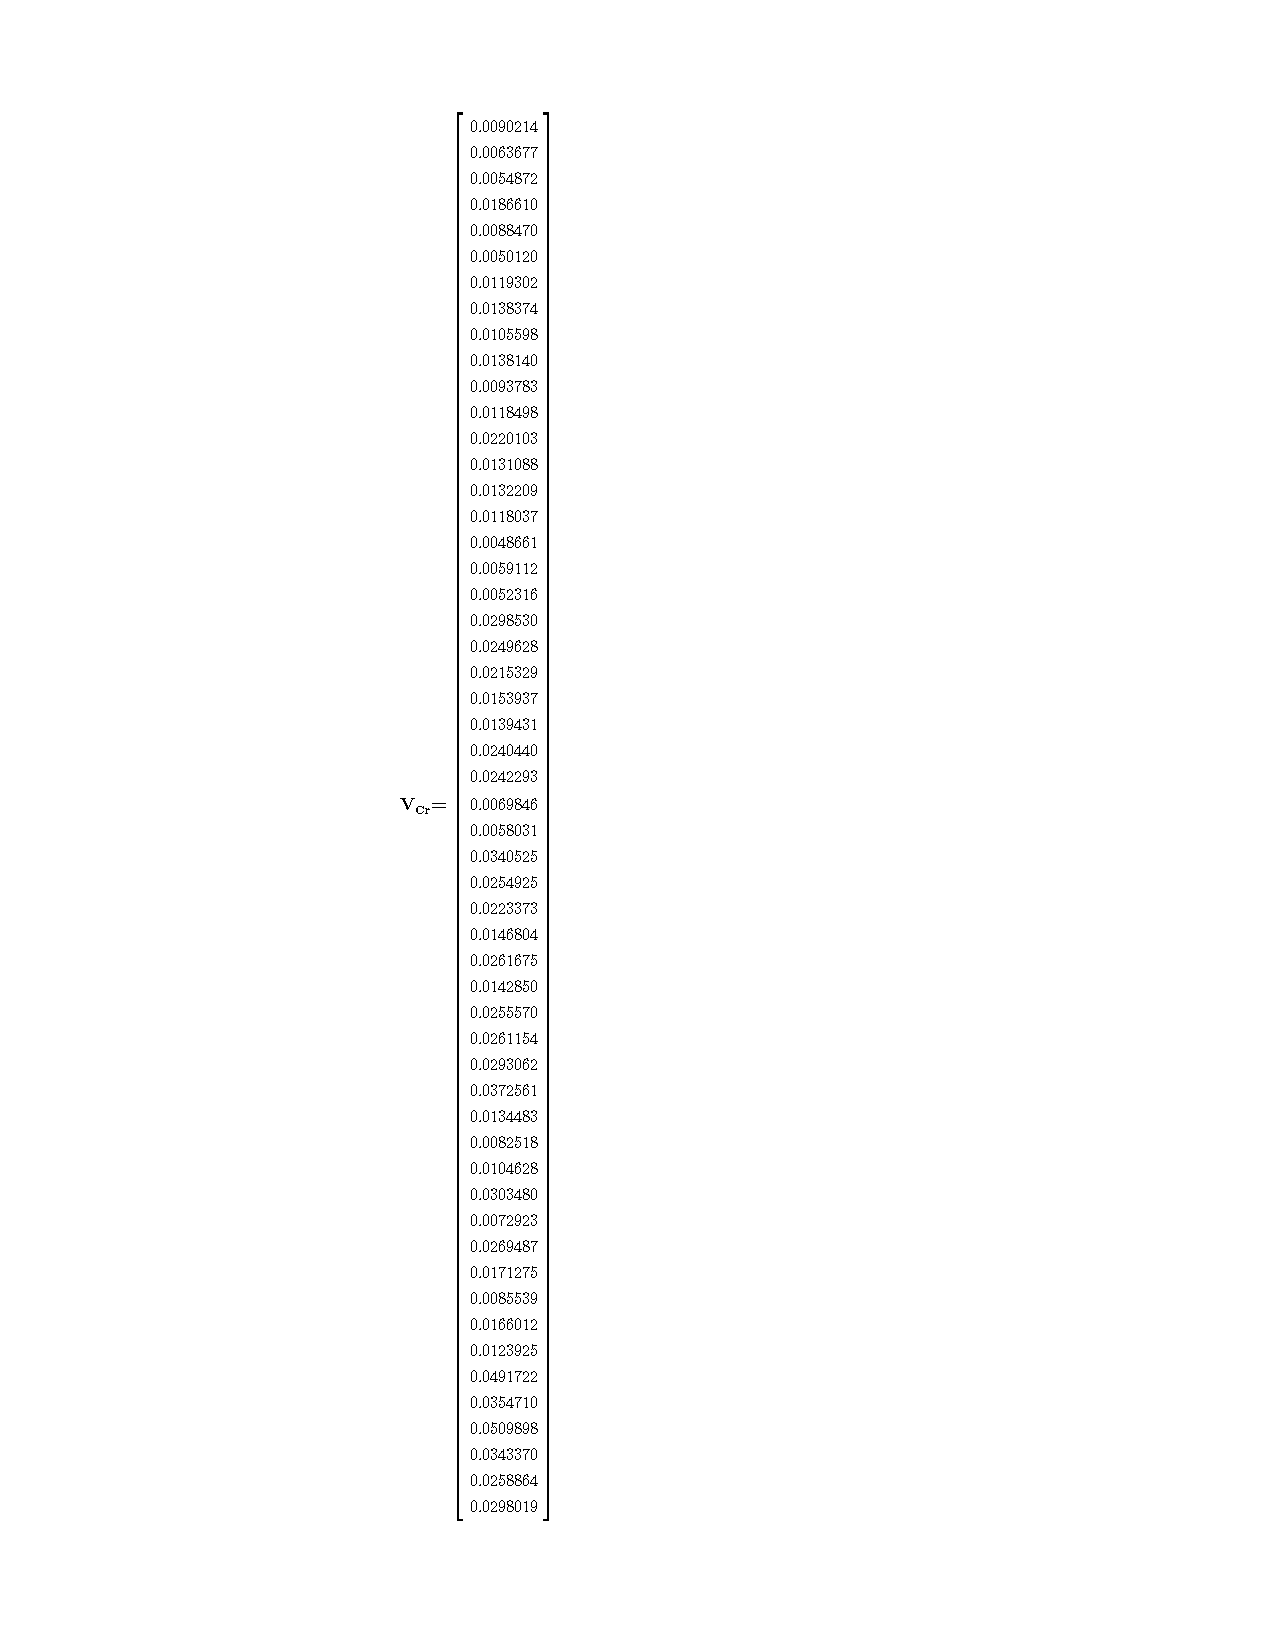
\includegraphics[width=15cm]{imagenes/VectorDePrioridadEx}
	\caption{Vector de prioridad de todos los criterios}
	\label{fig:VectorDePrioridadEx}
\end{figure}

\newpage
\begin{figure}[H]
	\centering
	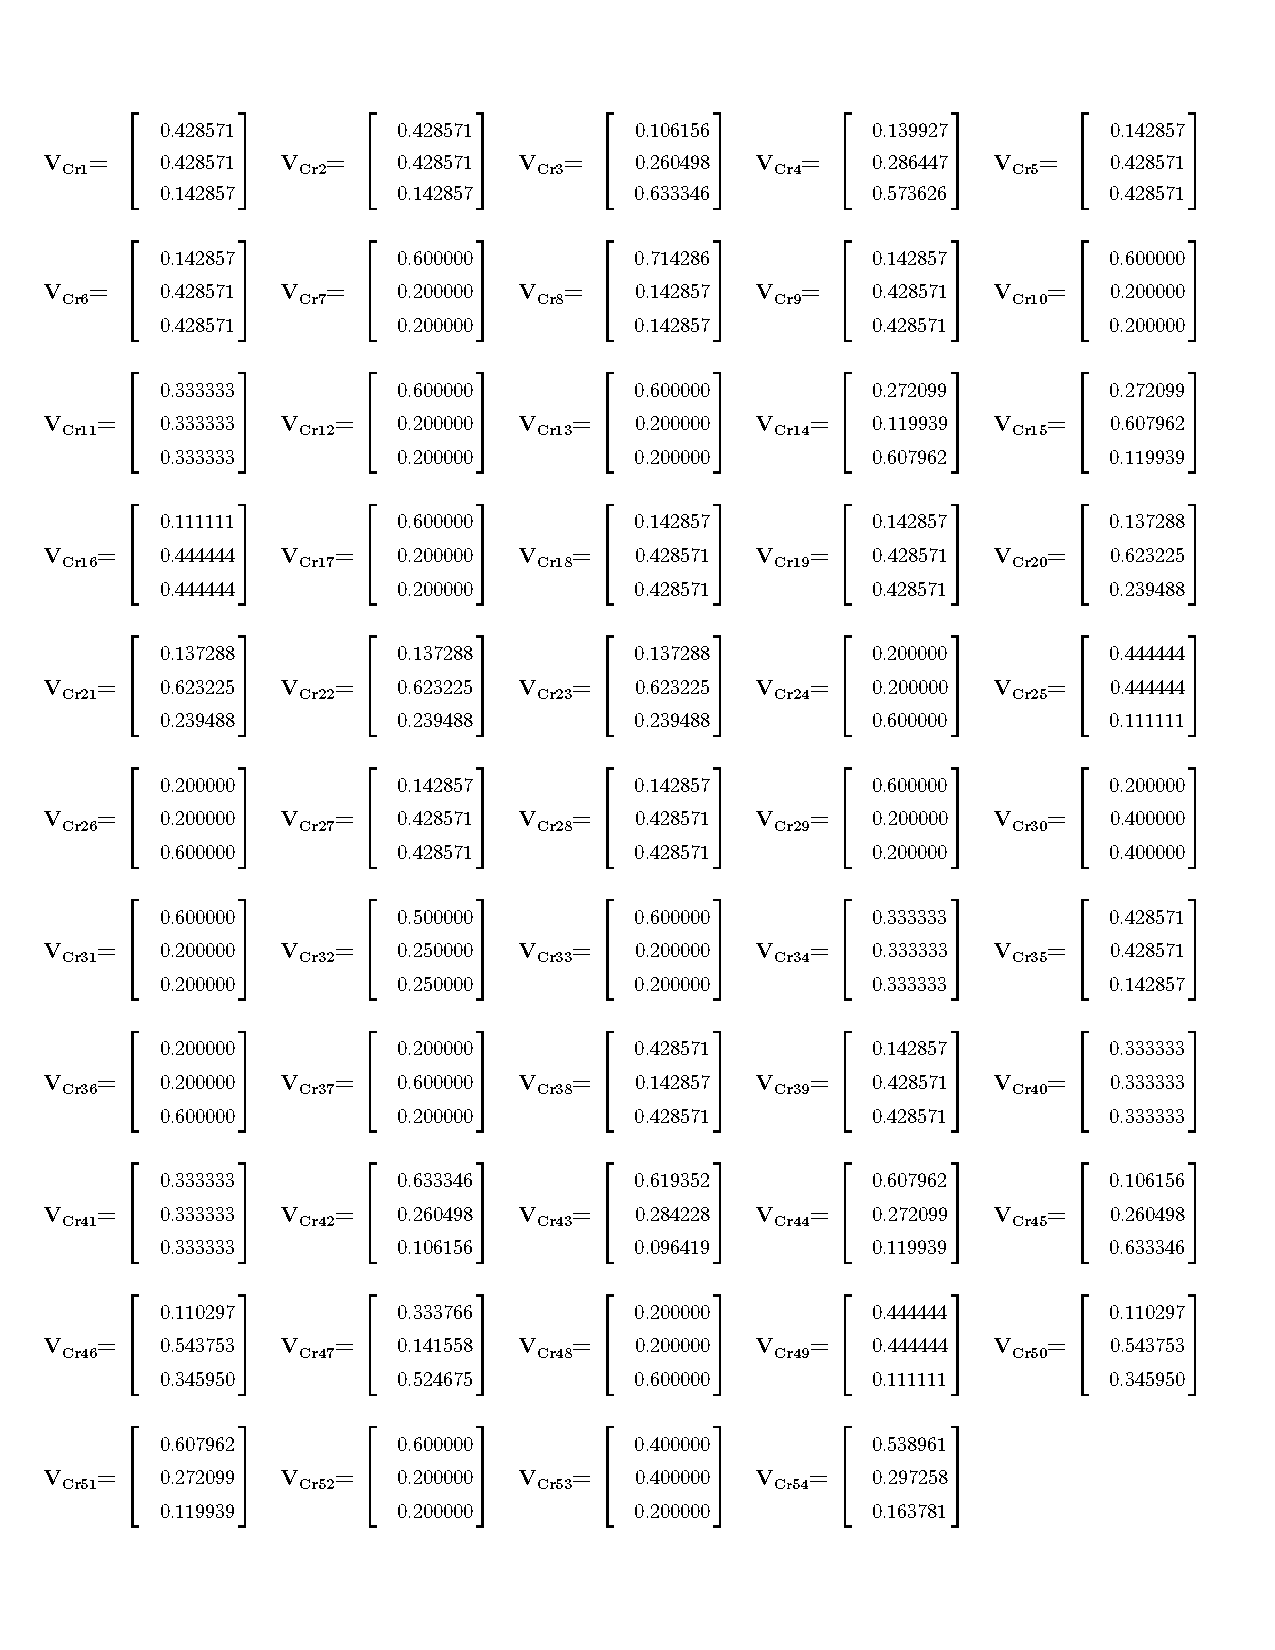
\includegraphics[width=15cm]{imagenes/54VectoresDePrioridadEx}
	\caption{Vector de prioridad de cada criterio.}
	\label{fig:54VectoresDePrioridadEx}
\end{figure}

\newpage
\begin{table}[H]
	\centering
	\caption{Diseños conceptuales propuestos y su valor y posición final.}
	\begin{tabular}{ccc}
		\hline
		& \textbf{Posición} & \textbf{Valor Final} \\
		\hline
		\hline
		\textbf{Diseño 1} & 1     & 0.3753656 \\
		\textbf{Diseño 2} & 2     & 0.3410145 \\
		\textbf{Diseño 3} & 3     & 0.2836199 \\
		\hline
	\end{tabular}%
	\label{tab:resultado AHP1}%
\end{table}%

\newpage
\begin{figure}[H]
	\centering
	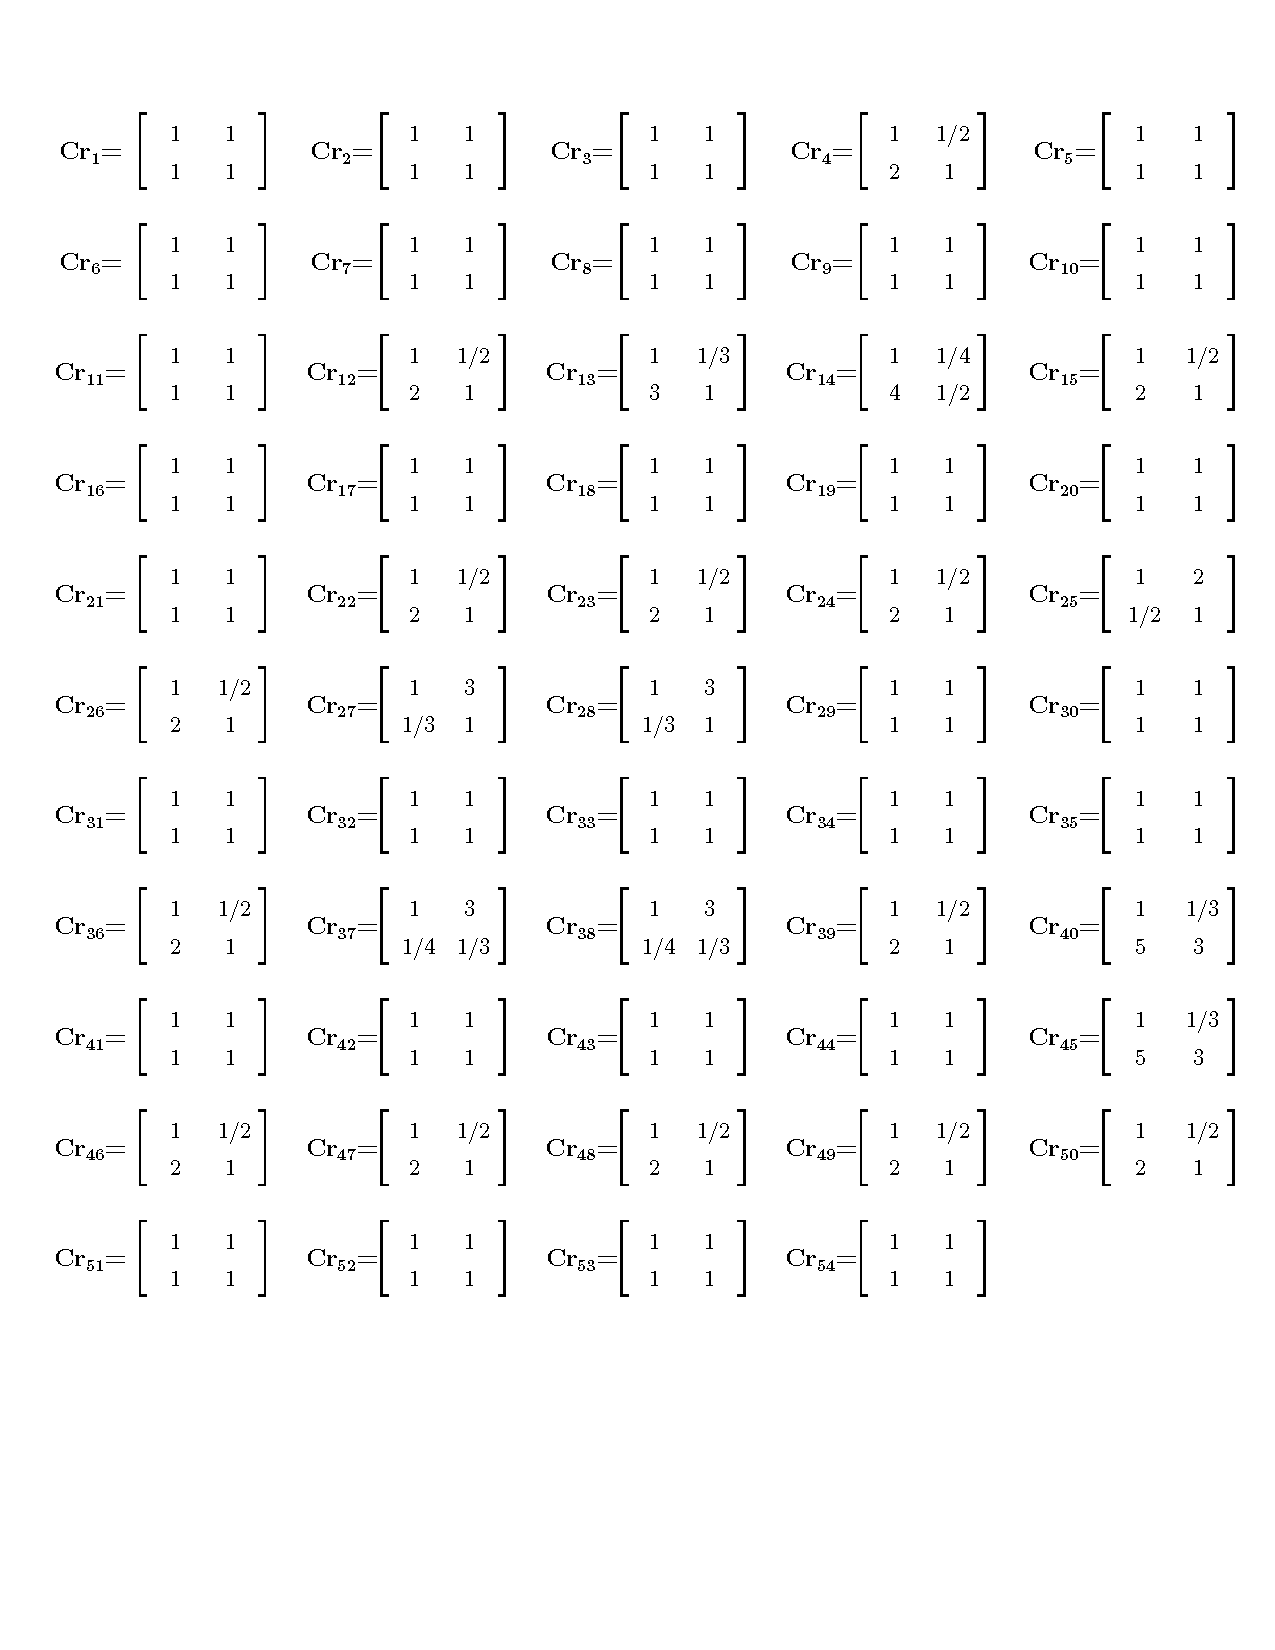
\includegraphics[width=14.5cm]{imagenes/54MatricesNormalMejoradoEx}
	\label{fig:MNormal1Ex1}
\end{figure}

\newpage
\begin{figure}[H]
	\centering
	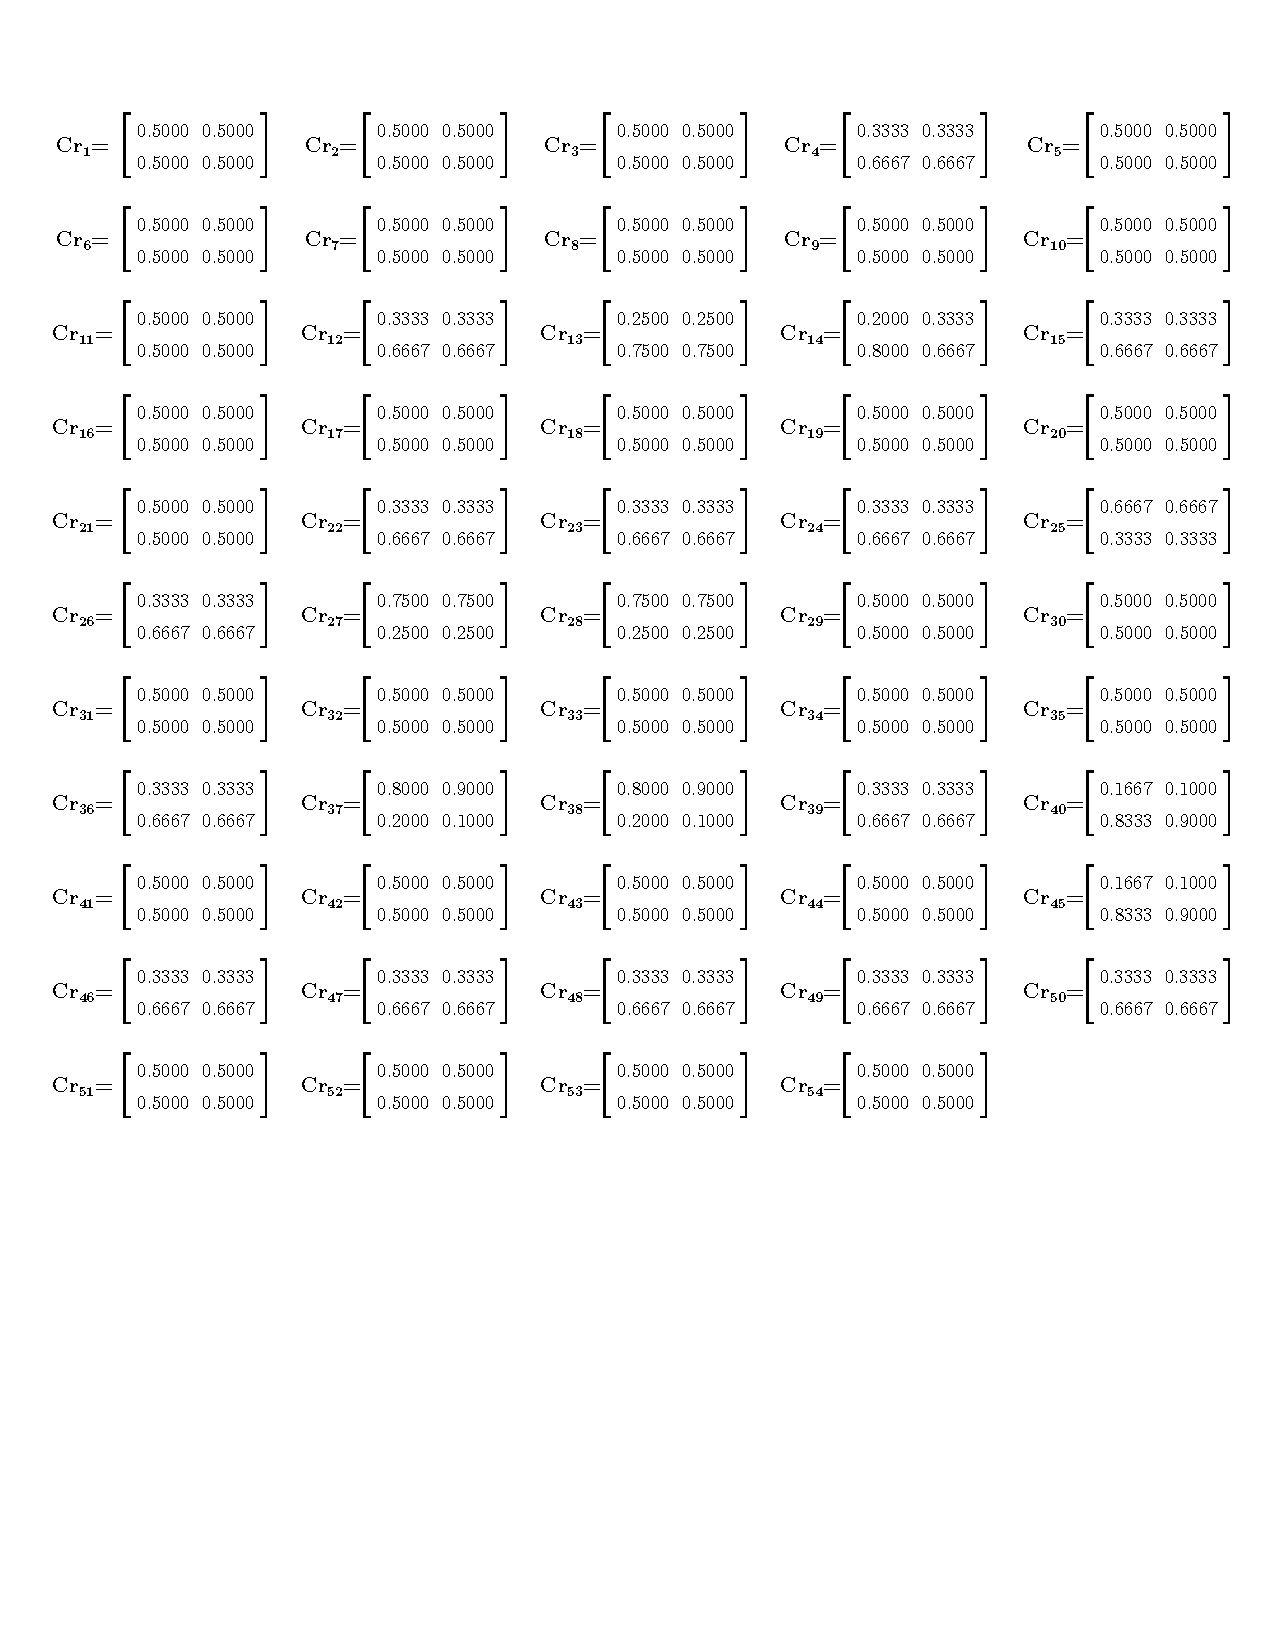
\includegraphics[width=15cm]{imagenes/54MatricesNormalizadoMejoradoEx}
	\label{fig:54Matrices}
\end{figure}

\newpage
\begin{figure}[H]
	\centering
	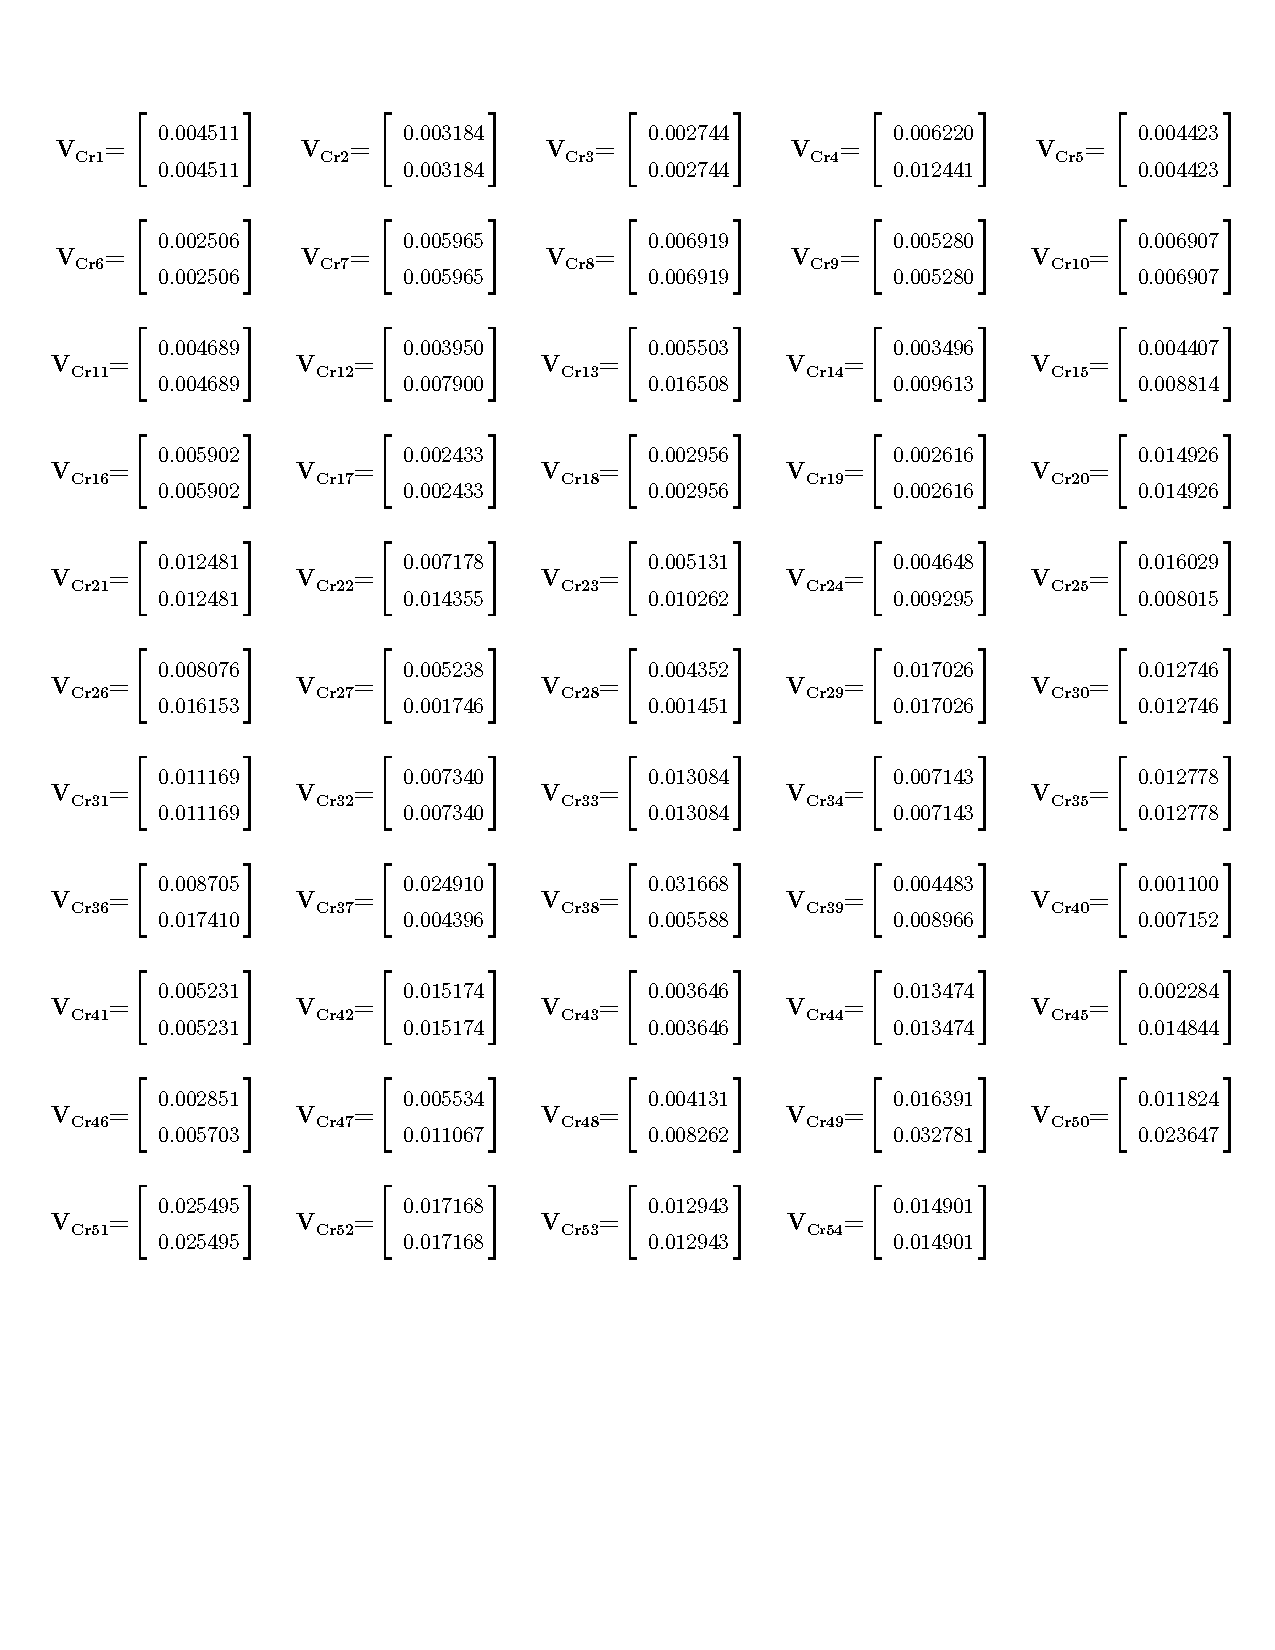
\includegraphics[width=14.5cm]{imagenes/54VectoresDePrioridadMejoradoEx}
	\label{fig:54VectoresDePrioridadEx1}
\end{figure}

\newpage
\begin{table}[H]
	\centering
	\caption{Valor y posición final del diseño conceptual ganador y diseño mejorado.}
	\begin{tabular}{ccc}
		\hline
		& \textbf{Posición} & \textbf{Valor Obtenido} \\
		\hline
		\hline
		\textbf{Diseño Ganador} & 2     & 0.4658699 \\
		\textbf{Diseño Mejorado} & 1     & 0.5341301 \\
		\hline
	\end{tabular}%
	\label{tab:finalmejorado}%
\end{table}%

\bigskip

%%%%%%fin del archivo
\endinput 